\chapter{Web data mining}
\section{Waarom data mining}
Met de opkomst van het internet, of meer bepaald het \emph{World Wide Web}, is er een explosie aan nieuwe data beschikbaar gekomen. Het web is een onderdeel geworden van het dagelijkse leven waarbij miljarden mensen met elkaar verbonden zijn via biljoenen documenten. Deze documenten zijn aan elkaar gelinkt via hyperlinks. Hierdoor is een nieuw soort maatschappij ontstaan: de virtuele maatschappij. 

Ondanks deze grote hoeveelheid nieuwe info is er een fenomeen ontstaan waarbij er een grote hoeveelheid data beschikbaar is die eigenlijk niet gebruikt wordt: de \emph{data gap}. De opslag van gegevens wordt steeds goedkoper, maar het analyseren van de data blijkt niet eenvoudig.

Er zijn drie grote elementen die de analyse moeilijk maken. Een eerste component is dat de data, beschikbaar op het internet, vaak geen vaste structuur heeft. Men moet dus eerst de data herwerken zodat men een vast patroon heeft dat gebruikt wordt in een bepaald algoritme.
Een tweede probleem is dat de data vaak veel ruis bevat, data die men niet nodig heeft. 
Tot slot is de data steeds veranderend: het is dynamisch.

Om deze grote hoeveelheid data toch te verwerken gebruikt men \emph{web data mining}. Dit is een automatische manier om informatie en kennis te extraheren uit het web. Deze techniek heeft 3 toepassingen: 
\begin{itemize}
  \item \textbf{Web content mining}: Het analyseren van data op basis van de inhoud van webpagina's.
  \item \textbf{Web usage mining}: Het analyseren van gedragspatronen op basis van de gebruikers logbestanden.
  \item \textbf{Web structure mining}: Het analyseren van het data op basis van hyperlinks.
\end{itemize}
\section{Data mining}
Voor we verder ingaan op het concept van web mining, bekijken we eerst \emph{data mining}. Data mining is het proces om patronen of kennis te ontdekken in databronnen. Het staat daarom ook bekend als KDD: \emph{Knowledge discovery in databases}. Dit proces is multidisciplinair en beslaat domeinen zoals \emph{machine learning}, statistiek, databanken, visualisatie \dots  Het proces is samengevat in de volgende figuur:

\begin{figure}
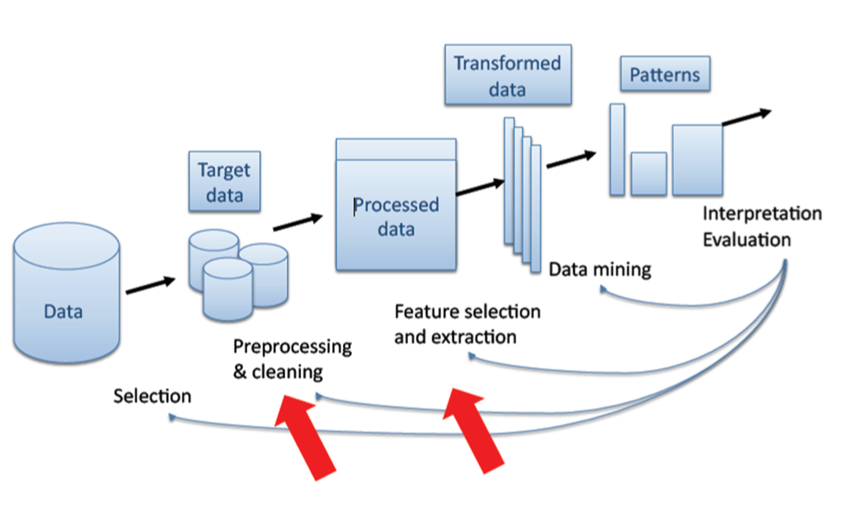
\includegraphics[]{res/kdd_process.png}
\caption{Het data mining proces.}
\end{figure}
Zoals we zien bestaat dit proces uit meerdere stappen.

\begin{enumerate}
\item Eerst wordt de data verzameld. Dit kan uit een database komen of kan bestaan uit verzameling van allemaal bronnen
\item In de tweede stap wordt een selectie gemaakt uit de data. Stel bijvoorbeeld dat we tweets analyseren. Indien we dit opvragen, dan krijgen we extra metadata zoals de locatie en of de tweet een antwoord is op iemand anders. We kunnen er dan voor kiezen om enkel tweets te selecteren die geen antwoord zijn.
\item Vervolgens is er de \emph{data cleaning}-stap. Hierbij wordt ontbrekende info aangevuld of wordt er data weggelaten indien blijkt dat deze niet bruikbaar is.
\item Nadat er enkel schone data overblijft moet deze nog worden omgezet naar data die gebruikt kan worden voor mining. Hierbij gebruikt men technieken zoals aggregatie van data, normalisatie.
\item De data is uiteindelijk klaar voor \emph{data mining}. Hierbij worden technieken zoals clustering en \emph{association} toegepast zodat er patronen kunnen vormen in de data.
\item Vervolgens wordt de data mining ge\"evalueerd en eventueel gevisualiseerd. 
\item Uiteindelijk wordt er gekeken of de data effectief nuttig is en tot meer kennis leidt.
\end{enumerate}
Merk op dat dit proces niet lineair is. Stel dat in stap 6 blijkt dat de mining slechte resultaten oplevert, dan kan men terugkeren naar de vorige stappen en kijken of er bijvoorbeeld geen nieuwe selectie gemaakt moet worden. Dit proces gaat door tot men resultaten bereikt waardoor men effectief kennis bijkrijgt.

Data mining bestaat dus uit een aantal technieken die in deze cursus besproken zullen worden. Hier onderscheid men onder andere:
\begin{itemize}
\item Supervised learning (\textasciitilde classificatie): Hierbij beschikt men over een reeds geclassificeerde database waarmee het algoritme kan leren en een database om het algoritme te testen.
\item Unsupervised learning(\textasciitilde clustering): Een groep van algoritmen waarbij het algoritme zelf bijleert over de dataset.
\item Association rule mining: Hierbij maakt men gebruik van technieken zoals: stel dat gebruiker 1 A en B koopt, en gebruiker 2 koopt A. Wat is dan de kans dat gebruiker 2 ook B zal kopen?
\item Sequential pattern mining: Een voorbeeld hiervan zijn DNA sequences waarbij blijkt dat sommige combinaties vaak voorkomen.
\end{itemize}
\section{Data mining vs Web mining}
\emph{Data mining} werkt dus in op gestructureerde data. Dit is dus een probleem voor de data verzamelt op het web omdat dit vaak ongestructureerd is. Hoe meer structuur er is in de data, hoe rijker en complexer de query's kunnen zijn. Wegens deze verschillen maakt men dus een onderscheid tussen \emph{web mining} en \emph{data mining}. Enkele voorbeelden van \emph{web mining} zijn:
\begin{itemize}
\item Tekst zoals contact info halen uit webpagina's
\item Video's uit webpagina's halen
\item Tabellen op bijvoorbeeld Wikipedia gebruiken om een analyse uit te voeren.
\end{itemize}
\newpage
\section{Besluit}
Algemeen kan men dus stellen dat web content mining een brede waaier is waarbij data mining ook gebruikt kan worden. De technieken die men hierbij onderscheid zijn:
\begin{itemize}
\item Unstructured data mining(=information retrieval)
\item Structured data mining op tabellen en databanken
\item Semi-structured: er is wel iets van structuur, maar deze moet nog gedefinieerd worden
\item Multimedia mining
\end{itemize}
De structuur van de data bepaalt het type van algoritmen. Gestructureerde data is vaak eenvoudiger te analyseren en leidt tot een grotere verzameling kennis.